\subsection{Modelos de Blinn y Blinn-Phong}
Empezamos viendo cómo las fuentes de luz presentes en la escena iluminan directamente la superficie. Hay multitud de modelos que simulan este comportamiento de forma más o menos realista, siendo uno de los más extendidos el renderizado basado en física (\textit{physically based rendering} o PBR). Sin embargo, este y otros acercamientos similares son utilizados cuando se requiere de un alto grado de fidelidad y adaptabilidad. Nosotros usaremos el modelo de reflexión de Blinn-Phong \cite{apuntes:ig}, también popular pero mucho más simple y computacionalmente menos costoso. A su vez este modelo se basa en el de Blinn, el cual pasamos a estudiar a continuación. \newline

Vamos a considerar que nuestra escena consta de los siguientes elementos.
\begin{itemize}
    \item La \textbf{isosuperficie} $S_{\phi}$ como único objeto a ser dibujado (aunque el modelo es válido para cualquier número de objetos en escena),
    \item Un \textbf{observador} que se encuentra en la posición $c_o\in\R^3$ mirando a un punto $p\in \R^3$,
    \item Un número finito $n$ de \textbf{fuentes de luz}. Llamaremos $l_i$ con $i=1,\dots, n$ a los vectores normalizados que apuntan desde $p$ a la posición de cada fuente.
\end{itemize}

Empecemos comprendiendo el fenómeno físico que tratamos de simular. La luz que generan las fuentes no es más que radiación electromagnética. De forma ideal, esta radiación se puede ver como un flujo en el espacio de partículas llamadas \textbf{fotones} que siguen trayectorias rectilíneas a la par que interaccionan con el entorno. Cada una de estas partículas tendrá una energía radiante única en función de su longitud de onda, que irá transfiriendo a aquellos objetos con los que interaccione.

\begin{definicion}[Radiancia]
    Dado un punto $p\in\R^3$, llamamos \textbf{radiancia} a la densidad de energía radiante por unidad de tiempo de los fotones que pasan por un entorno de $p$ en una determinada dirección $v\in\R^3$ con $\Vert v\Vert = 1$. La denotaremos $L(p,v)$, y será representada mediante una terna RGB no acotada. Podemos distinguir a su vez varios tipos de radiancia.
    \begin{itemize}
        \item \textbf{Radiancia emitida $\boldsymbol{L_E(p,v)}$:} radiancia que emite el propio objeto, también llamada emisividad. Normalmente es de intensidad baja y la consideraremos constante.
        \item \textbf{Radiancia incidente $\boldsymbol{L_{I}}(p,v)$:} radiancia que recibe el punto $p$ desde la dirección $v$. 
        \item \textbf{Radiancia reflejada $\boldsymbol{L_{R}}(p,v)$:} cantidad de la radiancia incidente en $p$ que se refleja en la dirección $v$. 
\end{itemize}
\end{definicion}

El objetivo del modelo será por tanto describir la radiancia que percibe el observador desde su posición en el punto $p$. Para ello, se llevan a cabo una serie de simplificaciones:
\begin{itemize}
    \item En un modelo físicamente correcto la luz reflejada en cada punto se dispersaría por el entorno, contribuyendo a la radiancia incidente en otros puntos de la escena. Sin embargo, nosotros no consideraremos la radiancia incidente que no provenga directamente de fuentes de luz. Incluso teniendo un solo objeto en escena como es nuestro caso este modelo es mejorable, pues el objeto puede reflejar radiancia sobre sí mismo. Por tanto, usaremos una radiancia ambiente constante $L_A$ para suplir esta iluminación indirecta.
    \item La radiancia se conserva en el espacio entre objetos.
    \item Las fuentes de luz son direccionales, de forma que no serán visibles en la escena. Además supondremos que emiten una radiancia constante $S_i$ para $i=1,\dots, n$.
    \item No se consideran objetos con transparencia.
\end{itemize}
Es natural pensar que la radiancia percibida en un punto $p\in \R^3$ será la suma de la radiancia que emita y la que sea capaz de reflejar. Así, teniendo en cuenta las consideraciones anteriores tenemos que
\begin{equation*}
    L(p,v) = L_A + L_E + \sum_{i=1}^n L_R(p,l_i).
\end{equation*}

Como $L_A$ y $L_E$ son constantes sólo nos falta estudiar cómo obtener la \textbf{radiancia reflejada} para cada fuente de luz. Para ello fijamos un índice $m\in \{1,\dots,n\}$ y suponemos a partir de ahora que $p\in S_{\phi}$, pues de lo contrario

\begin{equation*}
    L(p,v) = L_A,\ p\in \R^3\setminus S_{\phi},
\end{equation*}

ya que la única luz que se puede reflejar es la del ambiente, la cual ya está siendo considerada con $L_A$, y al trabajar únicamente con fuentes de luz direccionales $L_E=0$. \newline

Sabemos que cada objeto refleja la luz de manera distinta en función de su material y las propiedades de la fuente. Para representar este comportamiento definimos una función que indique la fracción de radiancia proveniente de $l_m$ que se refleja en un punto $p$ en la dirección $v$ para cada fuente de luz
\begin{equation*}
    f_r \colon \R^3\times \R^3\times \R^3 \to \R^3.
\end{equation*}

Así, la radiancia reflejada sería

\begin{equation*}
    L_R(p,v,l_m) = S_m\cdot f_r(p,v,l_m).
\end{equation*}

Podemos distinguir diferentes tipos de reflexión, cada uno contribuyendo de forma diferente a la radiancia reflejada final.

% donde $f_a$, $f_d$ y $f_e$ representan la fracción de radiancia reflejada para cada uno de los tipos de reflexión que podemos distinguir y listamos a continuación. 
\begin{itemize}
    \item \textbf{Reflexión ambiental:} cantidad de iluminación indirecta proveniente de la fuente de luz que refleja el objeto. Al igual que hicimos con $L_A$, tomaremos un valor constante $R_A$ para ella, de forma que la fracción de radiancia ambiental reflejada será
    \begin{equation*}
        f_{ra} =  R_A \in \R^3.
    \end{equation*}
    \item \textbf{Reflexión especular:} define cómo se refleja la luz en objetos brillantes teniendo en cuenta la posición de la fuente de luz y la del observador. Según la ley de refracción, el ángulo de incidencia de la luz será igual al de reflexión, luego podemos obtener la dirección de reflexión $r_m$ reflejando $l_m$ sobre el vector normal unitario en $p$ de la superficie, que llamaremos $N_p$. Así,
    
    \begin{equation*}
        r_m = 2(l_m\cdot N_p)N_p - l_m \in \R^3.
    \end{equation*}

    Sin embargo, solo queremos que haya reflejos en los puntos orientados hacia la fuente de luz y cuando $r_m$ haya sido reflejado en una dirección que el observador pueda apreciar, siendo la intensidad del reflejo mayor cuanto más alineado esté el observador con el vector reflejado. Esto equivale a que se cumpla
    \begin{equation*}
        N_p\cdot l_m >0 \quad \text{ y }\quad  R_m \cdot v>0.
    \end{equation*}
    Para controlar el color y la intensidad de los reflejos usaremos una radiancia $R_E$, de forma que podemos expresar la fracción de radiancia especular reflejada como
    \begin{align*}
        f_{re} \colon \R^3\times \R^3\times \R^3 &\to \R^3,\\
        (p,v,l_m) &\mapsto R_E \cdot \Max(0,l_m\cdot N_p) \cdot \Max(0,r_m \cdot v).
    \end{align*}
    \item \textbf{Reflexión difusa:} modela cómo se refleja la luz en objetos mates en función de la posición de la fuente de luz. Al contrario de lo que ocurre con la reflexión especular, debido a la irregularidad de la superficie del objeto la luz no se refleja en una sola dirección, haciendo que se disperse en direcciones impredecibles. Este comportamiento se simula a través de una radiancia $R_D$ que represente el valor promedio resultado de estos reflejos, y que consideraremos constante. Al igual que antes, solo queremos que el punto esté iluminado cuando esté de cara a la fuente de luz, obteniendo la mayor cantidad de luz cuando está alineado con la fuente. Así, la fracción de radiancia difusa será
    \begin{align*}
        f_{rd} \colon \R^3\times \R^3\times \R^3 &\to \R^3,\\
        (p,v,l_m) &\mapsto R_D\cdot \Max(0,l_m \cdot N_p).
    \end{align*}
\end{itemize}

\begin{figure}[ht!]
    \centering
    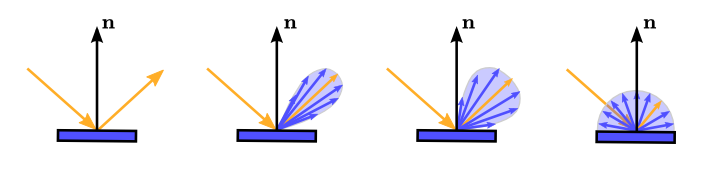
\includegraphics[width=0.85\textwidth]{Plantilla-TFG-master/img/glossyTodiffuse.png}
    \caption{Reflexión de un rayo en una superficie progresivamente más mate \cite{especular}}
    \label{fig:miss}
\end{figure}

\begin{observacion}
    Es necesario que los vectores $l_i$, $v$ y $N_p$ sean unitarios, pues de lo contrario su producto escalar no coincidiría con el coseno del ángulo que forman.
\end{observacion}

En vista de las definiciones anteriores, podríamos simplemente definir
\begin{equation*}
    f_r(p,v,l_m) = f_{ra}+f_{re}(p,v,l_m) + f_{r_d}(p,v,l_m).
\end{equation*}

De esta forma, para diferenciar entre un material totalmente mate como el yeso y uno especular como el metal bastaría tomar valores de $R_D$ y $R_E$ tal que $\Vert R_D\Vert \gg \Vert R_E\Vert$. Sin embargo, a la hora de comparar materiales especulares podríamos observar que aunque ambos generen zonas brillantes no lo hagan de la misma forma. Por ejemplo, tanto el mármol como el metal generan brillos sobre su superficie, pero en el caso del metal estos son más pequeños y brillantes debido a que se trata de un material más pulido. Por tanto, para añadir control sobre el tamaño e intensidad de estas zonas brillantes introducimos el \textbf{coeficiente de brillo} $\alpha \in \R$ en la expresión de $f_{re}$, de forma que cuanto mayor sea su valor más pequeños e intensos serán los brillos generados. En la \autoref{fig:parametrosEspecular} podemos ver el efecto que tienen $R_E,R_D$ sobre la radiancia reflejada \cite{especular}.\newline

\begin{definicion}
    Dado un objeto, definimos su \textbf{material} como la tupla $\{R_A,R_E,R_D,\alpha \}$.
\end{definicion}

Una vez asociado un material a $S_{\phi}$ podemos escribir la expresión final para $f_r$:

\begin{align}\label{eq:fr}
    f_r(p,v,l_i) &= f_{ra} &+\ & f_{re}(p,v,l_i) &+\ &f_{r_d}(p,v,l_i)\\
                 &= R_A    &+\ & R_E \cdot \Max(0,l_i\cdot N_p) \cdot \Max(0,r_i \cdot v)^{\alpha} &+\  &R_D\cdot \Max(0,l_i\cdot N_p). 
\end{align}

\begin{figure}[!h]
     \begin{minipage}[c]{0.45\linewidth}
        \centering
        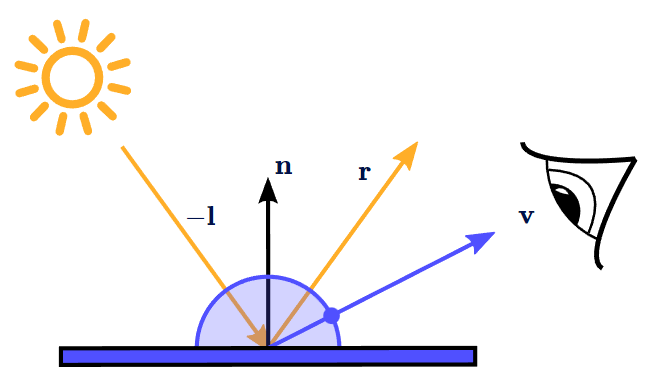
\includegraphics[width=0.95\textwidth]{Plantilla-TFG-master/img/ks0kd1.png}
        \caption{$\Vert R_E\Vert = 0$}
     \end{minipage}
     \begin{minipage}[c]{0.45\linewidth}
        \centering
        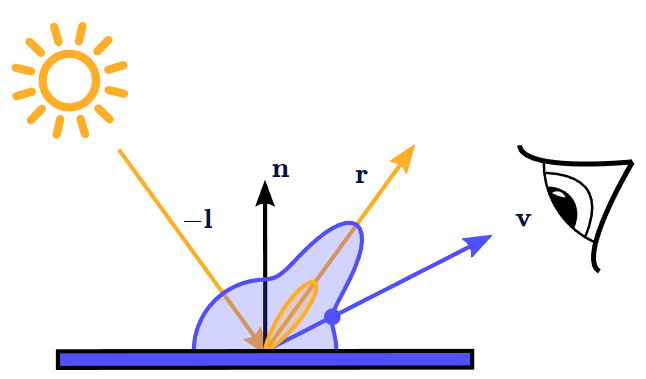
\includegraphics[width=0.95\textwidth]{Plantilla-TFG-master/img/ks1kd1.png}
        \caption{$\Vert R_E\Vert =\Vert R_D\Vert$ y $\alpha$ grande}
     \end{minipage}
     \begin{minipage}[c]{0.45\linewidth}
        \centering
        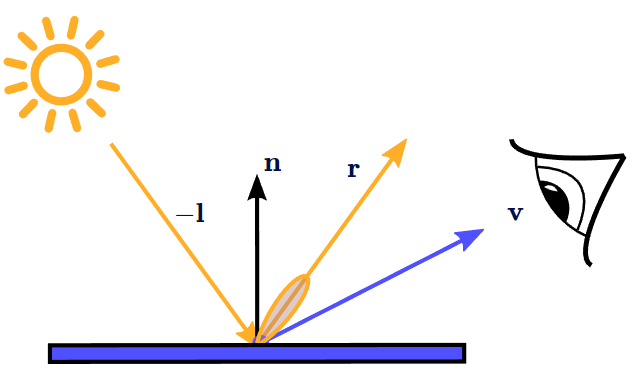
\includegraphics[width=0.95\textwidth]{Plantilla-TFG-master/img/ks1kd0.png}
        \caption{$\Vert R_D\Vert = 0$}
     \end{minipage}
     \begin{minipage}[c]{0.45\linewidth}
        \centering
        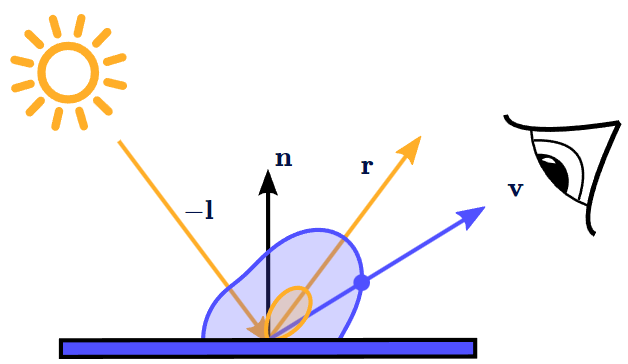
\includegraphics[width=0.95\textwidth]{Plantilla-TFG-master/img/ks1kd1a0.png}
        \caption{$\Vert R_E\Vert =\Vert R_D\Vert$ y $\alpha$ pequeño}
     \end{minipage}
     % \begin{minipage}[c]{0.45\linewidth}
     %    \centering
     %    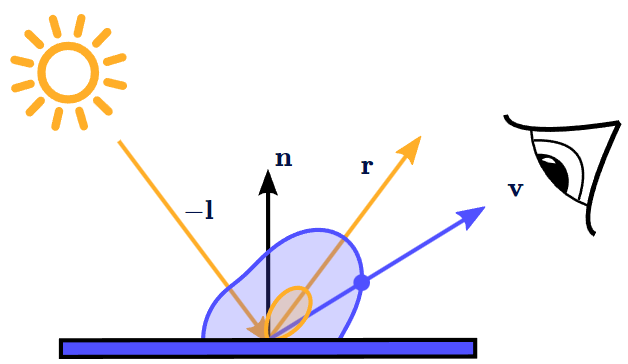
\includegraphics[width=0.95\textwidth]{Plantilla-TFG-master/img/ks1kd1a0.png}
     %    \caption{$k_s = 1$ y $k_d = 0$}
     % \end{minipage}
     \caption{Ejemplo de distintos valores para $R_E,R_D$ y $\alpha$}
     \label{fig:parametrosEspecular}
\end{figure}

Recogemos los resultados obtenidos en la siguiente definición.
\begin{definicion}[Modelo de Blinn]\label{def:blinn} La radiancia percibida en el punto $p\in\R^3$ desde la dirección $v\in\R^3$ con $\Vert v\Vert = 1$ según el modelo de Blinn viene dada por
    \begin{equation*}
        L(p,v) = L_A+L_E+ \sum_{i=0}^n S_i \Bigg[ k_aR_A + \Max(0,l_i\cdot N_p) \Big( k_dR_D + k_eR_E\cdot \Max(0,r_i\cdot v) \Big) \Bigg],
    \end{equation*}

    donde:
    \begin{itemize}
        \item $n \in \N$ es el número de fuentes de luz y $l_i \in R^3$ es el vector normalizado que apunta a $p$ desde cada una de ellas,
        \item $L_A,L_E \in \R^3$ son ternas RGB no acotadas representando la radiancia ambiente y emitida respectivamente,
        \item $S_i \in \R^3$ es una terna RGB no acotada representando la radiancia emitida por la fuente de luz $i$-ésima,
        \item $\alpha \in \R$ es el coeficiente de brillo,
        \item $R_A,R_D,R_E \in \R^3$ son ternas RGB (no acotadas) representando la radiancia reflejada de forma ambiental, difusa y especular respectivamente,
        \item $N_p$ es el vector normal de la superficie en $p$ y $r_i$ es el vector $l_i$ reflejado sobre $N_p$.
    \end{itemize}
\end{definicion}

En 1975 Phong introdujo una variante a este modelo \cite{phong} que hoy conocemos como \textbf{modelo de Blinn-Phong}. Su única diferencia con el de Blinn consiste en el uso del llamado \textit{halfway vector}
\begin{equation*}
    h_m = \frac{l_m + v}{\Vert l_m + v\Vert}.
\end{equation*}

Ahora, en lugar de usar el valor $r_m\cdot v$ hacemos que el brillo sea proporcional al coseno del ángulo entre $h_m$ y $N_p$, de forma que no depende del punto $p$ y solo necesita ser calculado una vez. En la \autoref{fig:phong} podemos ver el comportamiento de $h_m$ para distintas configuraciones de $l_m$ y $v$.
\begin{figure}[!h]
     \begin{minipage}[c]{0.32\linewidth}
        \centering
        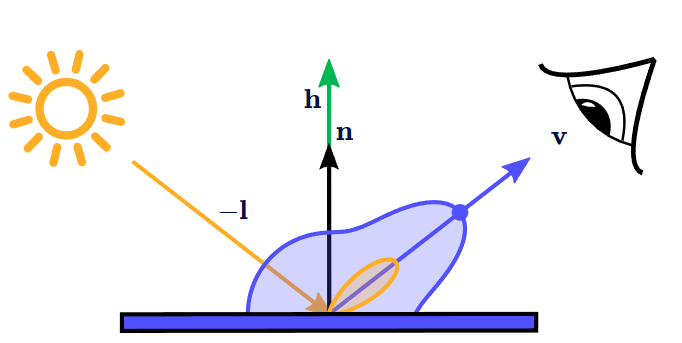
\includegraphics[width=0.95\textwidth, align=b]{Plantilla-TFG-master/img/phong1.png}
     \end{minipage}
     \begin{minipage}[c]{0.32\linewidth}
        \centering
        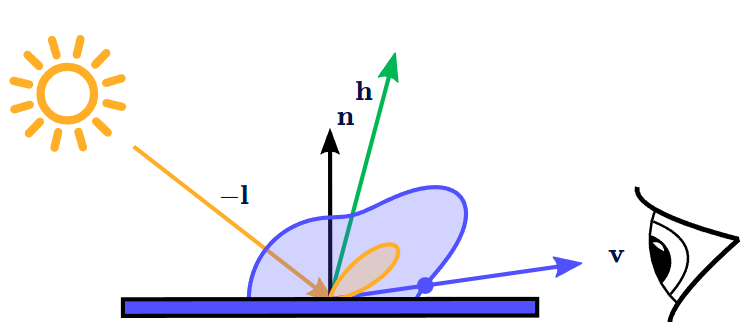
\includegraphics[width=0.95\textwidth, align=b]{Plantilla-TFG-master/img/phong2.png}
     \end{minipage}
     \begin{minipage}[c]{0.32\linewidth}
        \centering
        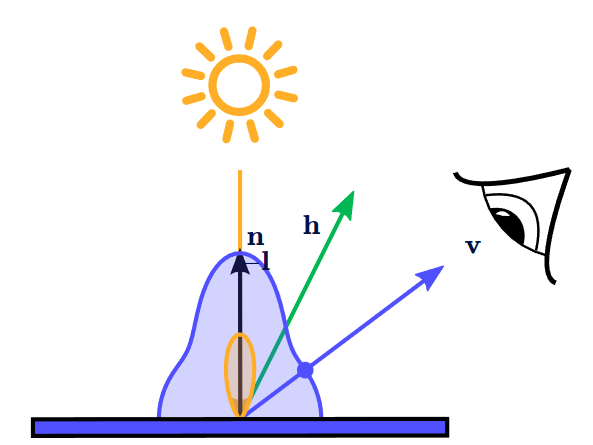
\includegraphics[width=0.95\textwidth, align=b]{Plantilla-TFG-master/img/phong3.png}
     \end{minipage}
     \caption{Comportamiento de  $h_m$ con $\Vert R_S\Vert =\Vert R_D\Vert$}
     \label{fig:phong}
\end{figure}

Aunque pueda parecer una simplificación del modelo de Blinn, lo cierto es que produce resultados más convincentes que este. En particular, mientras que el modelo de Blinn siempre produce brillos redondos en superficies planas, el de Blinn-Phong los genera con una forma más elíptica cuando se observa la superficie desde un ángulo acusado, como se observa en la \autoref{fig:difBlinn}. 

\begin{figure}[!h]
     \begin{minipage}[c]{0.49\linewidth}
        \centering
        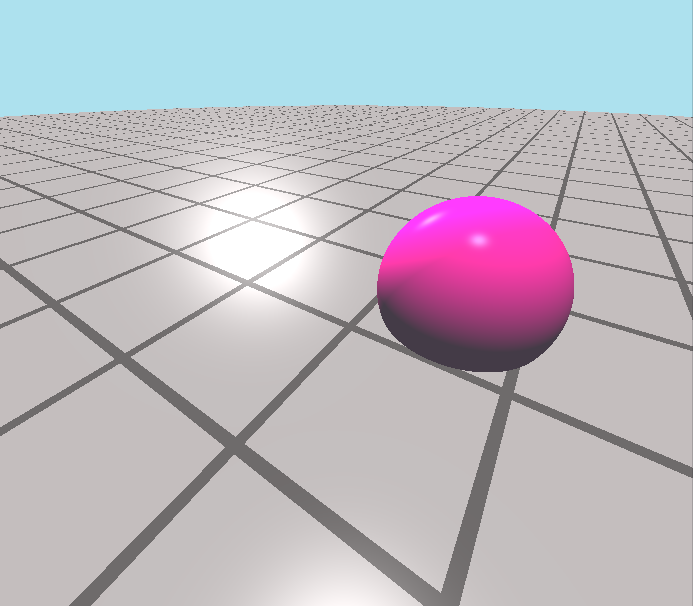
\includegraphics[width=0.9\textwidth]{Plantilla-TFG-master/img/compB.png}
        \caption{Blinn}
     \end{minipage}
     \begin{minipage}[c]{0.49\linewidth}
        \centering
        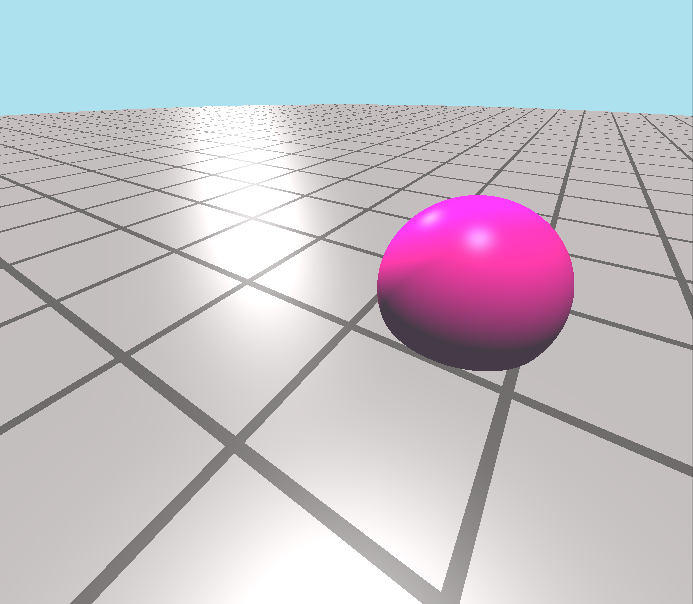
\includegraphics[width=0.9\textwidth]{Plantilla-TFG-master/img/compBP.png}
        \caption{Blinn-Phong}
     \end{minipage}
     \caption{Zonas brillantes en modelos de Blinn y Blinn-Phong}
     \label{fig:difBlinn}
\end{figure}

\begin{definicion}[Modelo de Blinn-Phong]
    En el contexto de la \autoref{def:blinn}, la radiancia percibida en el punto $p\in\R^3$ desde la dirección $v\in\R^3$ con $\Vert v \Vert = 1$ según el modelo de Blinn-Phong viene dada por
    \begin{equation*}
        L(p,v) = L_A+L_E+ \sum_{i=0}^n S_i \Bigg[ k_aR_A + \Max(0,l_i\cdot N_p) \left( k_dR_D + k_eR_E\cdot \left(N_p\cdot \frac{l_i + v}{\Vert l_i + v\Vert} \right)^{\alpha} \right) \Bigg],
    \end{equation*}
\end{definicion}

Ya podemos darle forma a las funciones \texttt{DibujarSuperficie} y \texttt{DibujarFondo} usadas en la \autoref{a:spheretracing}, suponiendo que pasamos como \textit{uniforms} los parámetros del material y los valores $l_i$ y $S_i$ para cada $i=1,\dots, n$.
\begin{figure}[ht!]
    \centering
    
       \begin{algorithm}[H]
            \caption{DibujarSupercicie}
                \KwData{punto $p$, dirección del rayo $v$, distancia $\phi(p)$}
                $L \gets L_A$ \Comment{Radiancia final}
                \For{$i \in \{1,\dots, n\}$} {

                    
                    $h \gets normalizar(L_i - v)$ \Comment{Observador en dirección opuesta a la del rayo}
                    
                    $N_p \gets calcularNormal(p)$
                    
                    $NLi \gets \Max(0,\ N_p\cdot l_i)$
                    
                    $NH \gets \Max(0,\ N_p \cdot h)$\newline

                    $f_{ra} = R_A$
                    
                    $f_{rd} = NLi\cdot R_D$
                    
                    $f_{re} = NLi \cdot R_E \cdot NH^{\alpha}$\newline

                    $L \gets L + S_i\cdot (f_{ra} + f_{rd} + f_{re})$
                }

                \Return{$L$}
        \end{algorithm}
    \begin{algorithm}[H]
            \caption{DibujarFondo}
                \Return{$L_A$}
        \end{algorithm}

        \caption{Implementación de las funciones \texttt{DibujarSuperficie} y \texttt{DibujarFondo}}
\end{figure}

Sólo queda un asunto por tratar. A la vista de la expresión de $f_r$ \eqref{eq:fr} y del código anterior, somos capaces de calcular todos los valores a excepción de uno, el del vector normal. Debido a que no trabajamos con vértices, deberemos de buscar métodos diferentes a los usuales para obtenerlo.

\subsubsection{Cálculo del vector normal}
Empezamos introduciendo una propiedad para ciertas funciones $\phi:\R^3\to\R$ que nos será útil más adelante. 

\begin{definicion}
    Una función $\phi\colon \R^3 \to \R$ es diferenciable en $t_0 \in \R^3$ si existe una función lineal $L\colon \R^3\to \R$ tal que
    \begin{equation*}
        \lim_{h\to 0}\frac{\vert \phi(t_0+h)-\phi(t_0) - L(h)\vert}{\Vert h\Vert} = 0.
    \end{equation*}
\end{definicion}

Si una función es diferenciable existen todas sus derivadas parciales, lo que nos permite hacer la siguiente definición.
\begin{definicion}
  Definimos el \textbf{gradiente} de una función implícita diferenciable $\phi\colon \R^3\to\R$ como $\nabla\phi = \left(\frac{\partial \phi}{\partial x}, \frac{\partial \phi}{\partial y}, \frac{\partial \phi}{\partial z}\right)$.
\end{definicion}

\begin{proposicion}\label{p:gradient_perp}
  Sea $\phi\colon \R^3\to \R$ diferenciable. Entonces $\nabla\phi$ es perpendicular a $S_\phi$.
\end{proposicion}

\begin{proof}
  Sea $s\in S_\phi$ arbitrario. Tomamos una curva parametrizada:
  \begin{align*}
    \alpha \colon [0,1] & \to S_\phi                             \\
    t                   & \mapsto \left(x(t), y(t), z(t) \right)
  \end{align*}

  cumpliendo $\alpha(t_0)=s$ para algún $t_0\in [0,1]$. Veamos que $\nabla\phi(s) \perp \alpha$:

  \begin{align*}
    \alpha(t)\subset S_\phi & \implies \phi(\alpha(t))=0\\
                            & \implies \nabla\phi(\alpha(t)) = \frac{\partial{F}}{\partial{x}}\frac{dx}{dt} + \frac{\partial{F}}{\partial{y}}\frac{dy}{dt} + \frac{\partial{F}}{\partial{z}}\frac{dz}{dt} = 0 \\
                            & \implies \langle \nabla\phi(x,y,z), \alpha'(t)\rangle = 0 \implies \langle \nabla\phi(x,y,z), \alpha'(t_0)\rangle = 0
  \end{align*}

    Por tanto $\nabla\phi(s)$ es perpendicular al vector tangente de $\alpha$ en $s$, que a su vez está contenido en el plano tangente de $S_\phi$ en $s$. Por tanto $\nabla\phi(s) \perp S_\phi$.
\end{proof}

Hemos visto que calcular el vector normal en cualquier punto equivale a calcular $\nabla\phi$. Sin embargo, no tenemos certeza que nuestro SDF $\phi$ vaya a ser diferenciable en todo su dominio. De hecho, en la \autoref{sec:operaciones} hemos visto varios ejemplo de operaciones que darían como resultado SDF no derivables, como aquellas que usan el valor absoluto. Vamos a ver la información que tenemos acerca de los puntos en los que $\phi$ no es derivable \cite{derivWiki}.

\begin{lema}
    Sea $\phi:\R^3\to \R$ un SDF. Entonces $\phi$ es lipschitziana de constante $L=1$.
\end{lema}
\begin{proof}
    Sean $p$ y $q\in \R^3$. Usando la \autoref{def:sdf}, para todo $s\in S_{\phi}$ se tiene
    \begin{align*}
        \phi(p) &\le \Vert p-s\Vert = \Vert p-q+q+s\Vert \le \Vert p-q\Vert + \Vert q-s\Vert\\[10pt] 
        &\implies \phi(p) - \Vert p-q\Vert \le \Vert q-s \Vert \implies  \phi(p) - \Vert p-q\Vert \le \Inf_{s\in S_{\phi}}(\Vert q-s \Vert) = \phi(q)\\[10pt]
        &\implies \phi(p) - \phi(q) \le \Vert p-q \Vert
    \end{align*}

    De forma análoga podemos ver que $\phi(q) - \phi(p) \le \Vert q-p \Vert$, luego
    \begin{equation*}
        \vert \phi(p) - \phi(q)\vert \le 1\cdot \Vert p-q\Vert.
    \end{equation*}
\end{proof}

\begin{proposicion}[Teorema de Rademacher]
    Sea $U$ un abierto de $\R^3$ y $f:U\to \R$ lipschitziana. Entonces $f$ es diferenciable en casi todo punto de $U$.
\end{proposicion}

Tenemos por tanto asegurado que $\phi$ será diferenciable en casi todo punto de $\R^3$. No obstante, podemos concretar aún más dónde están los puntos de conflicto \cite{dif1} \cite{dif2}. Para ello necesitaremos introducir el concepto de esqueleto de una superficie \cite{derivWiki}.
\begin{definicion}
    Sea $\phi \colon \R^3\to \R$ un SDF. Llamamos \textbf{esqueleto} de $S_{\phi}$ al conjunto de puntos de $\R^3$ cuya distancia a la superficie puede obtenerse como la distancia a dos o más puntos distintos de $\delta S_{\phi}$:
    \begin{equation}
        \epsilon(S_{\phi}) = \{p\in \R^3 : \phi(p) = \Vert p-q\Vert = \Vert x-r\Vert,\ q,r\in \delta(S_{\phi}),\ q\neq r \}.
    \end{equation}
\end{definicion}

\begin{teorema}
    Sea $\Omega \subseteq \R^3$ un conjunto abierto con frontera diferenciable y $\phi_{\Omega} \colon \R^3\to \R$ un SDF. Entonces $\phi_{\Omega}$ es diferenciable en un entorno tubular $U$ de $\delta \Omega$. Es más, para cada $p\in \R^3$ se cumple una se las siguientes propiedades.
    \begin{enumerate}
        \item $p\in \delta \Omega$ y $\phi_{\Omega}$ es diferenciable en $p$ con $\nabla S_{\phi(p)} = N_p$,
        \item $p\notin \delta \Omega$ y $\phi_{\Omega}$ es diferenciable en $p \iff p\in \R^3\setminus \delta\Omega$, en cuyo caso
        \begin{equation*}
            \nabla \phi_{\Omega}(p) = \frac{q-p}{\phi_{\Omega}(p)},
        \end{equation*}
        donde $q$ es el único punto de $\delta\Omega$ tal que $\phi_{\Omega}(p) = \Vert q-p\Vert$.
    \end{enumerate}
\end{teorema}

\begin{corolario}
    Todo SDF $\phi\colon \R^3\to \R$ satisface la ecuación de la eikonal 
    \begin{equation*}
        \Vert \nabla \phi(p)\Vert = 1
    \end{equation*}
    en todo punto $p$ donde sea diferenciable.
\end{corolario}

\begin{corolario}
    Todo SDF $\phi\colon \R^3\to \R$ es diferenciable en $p \iff p\in \R^3\setminus \epsilon(S_{\phi})$. 
\end{corolario}

A la vista de este resultado podemos diferenciar $\phi$ con tranquilidad, pues solo estamos interesados en estudiar el gradiente en puntos de $\delta\Omega$. Sin embargo, que el gradiente exista no significa que podamos o debamos obtenerlo de forma analítica. Si bien en muchos casos sería posible hacerlo de forma analítica, esto podría tener asociado un coste computacional que no podemos asumir. En su lugar, utilizaremos un método numérico aproximado que, sin ser el más preciso, produce buenos resultados y es rápido, haciendo uso únicamente de unas pocas evaluaciones de $\phi$. Antes de verlo repasamos un último concepto de análisis diferencial.

% TODO: ver si decir que podria calcularse fuera del shader pasanndo el string al shader y recompilando. Si no, ver si comentar algo de que hay que calcularlo cada frame, y por eso no podemos hacerlo analiticamente
% De ser derivable, podría ser una buena opción calcular el gradiente una única vez al momento de definir $\phi$, tras lo cual para obtener $N$ solo habría que realizar evaluaciones de dicho gradiente. Sin embargo, esto requeriría de varias comprobaciones previas, y aún necesitaríamos otro método para tratar las no diferenciables. Por ello nos decantaremos por un método numérico más sencillo que únicamente hará uso de evaluaciones de $\phi$.

\begin{definicion}
  Dada $\phi:\R^3\to \R$ diferenciable, $p = (x,y,z)$, $v\in \R^3$, definimos la \textbf{derivada direccional} en $p$ en la dirección $v$ a:
  \begin{equation*}
    \nabla_v f(p) = \nabla f(p) \cdot v = \frac{\partial{f}(p)}{\partial{x}}v_x + \frac{\partial{f}(p)}{\partial{y}}v_y + \frac{\partial{f}(p)}{\partial{z}}v_z
  \end{equation*}
\end{definicion}

Para el cálculo de cada parcial de $f$ podemos utilizar la definición de derivada. Por ejemplo, para la primera componente tendríamos
\begin{equation*}
  \frac{\partial{f}(p)}{\partial{x}} v_x = \lim_{h\to 0}\frac{f(p + (h,0,0)) - f(p)}{h} v_x
\end{equation*}

Ahora sí, tenemos todas las herramientas para aplicar el \textbf{método del tetraedro} \cite{article:tetra}, el cual se basa en evaluar $\phi$ en la dirección de los vértices de un tetraedro:

\begin{equation*}
    k_0 = (1,-1,-1),\quad k_1 = (-1,-1,1),\quad k_2=(-1,1,-1),\quad k_3=(1,1,1).
\end{equation*}

\begin{proposicion}[Método del tetraedro]
  Dado $p\in S_\phi$, una aproximación de su vector normal $N_p$ se obtiene normalizando el vector
  \begin{equation*}
    \hat{N_p} = \sum_{i=0}^3 k_i\cdot f(p + hk_i)\quad \text{, donde } h\approx 0.
  \end{equation*}
\end{proposicion}

\begin{proof}
  Por la proposición \autoref{p:gradient_perp}, basta comprobar que $\hat{N}$ es colineal a $\nabla \phi(p)$.

  \begin{align*}
    \hat{N} & = \sum_{i=0}^3 k_i\cdot f(p + hk_i) = \sum_{i=0}^3 k_i\cdot f(p + hk_i) - k_i\cdot f(p) = \sum_{i=0}^3 k_i\cdot \left[ f(p+hk_i) - f(p)\right]\\ &= h\sum_{i=0}^3 k_i \nabla_{k_i}f(x)
    = h\sum_{i=0}^3 k_i \cdot \left( k_i \cdot \nabla f(p)\right) = h\sum_{i=0}^3 (k_i\cdot k_i) \nabla f(p) = h\sum_{i=0}^3 \nabla f(p) = 4h\nabla f(p)
  \end{align*}

  donde hemos usado que $\sum_{i=0}^3 k_i = (0,0,0)$, $\sum_{i=0}^3 k_i\cdot k_i = (1,1,1)$ y que el producto escalar es un operador lineal.
\end{proof}